%%%%%%%%%%%%%%%%%%%%%%%%%%%%%%%%%%%%%%%
% Wenneker Resume/CV
% LaTeX Template
% Version 1.1 (19/6/2016)
%
% This template has been downloaded from:
% http://www.LaTeXTemplates.com
%
% Original author:
% Frits Wenneker (http://www.howtotex.com) with extensive modifications by
% Vel (vel@LaTeXTemplates.com)
%
% License:
% CC BY-NC-SA 3.0 (http://creativecommons.org/licenses/by-nc-sa/3.0/
%
%%%%%%%%%%%%%%%%%%%%%%%%%%%%%%%%%%%%%%

%----------------------------------------------------------------------------------------
%	PACKAGES AND OTHER DOCUMENT CONFIGURATIONS
%----------------------------------------------------------------------------------------

\documentclass[a4paper,12pt]{memoir} % Font and paper size

%%%%%%%%%%%%%%%%%%%%%%%%%%%%%%%%%%%%%%%%%
% Wenneker Resume/CV
% Structure Specification File
% Version 1.1 (19/6/2016)
%
% This file has been downloaded from:
% http://www.LaTeXTemplates.com
%
% Original author:
% Frits Wenneker (http://www.howtotex.com) with extensive modifications by 
% Vel (vel@latextemplates.com)
%
% License:
% CC BY-NC-SA 3.0 (http://creativecommons.org/licenses/by-nc-sa/3.0/)
%
%%%%%%%%%%%%%%%%%%%%%%%%%%%%%%%%%%%%%%%%%

%----------------------------------------------------------------------------------------
%	PACKAGES AND OTHER DOCUMENT CONFIGURATIONS
%----------------------------------------------------------------------------------------

\usepackage{XCharter} % Use the Bitstream Charter font
\usepackage[utf8]{inputenc} % Required for inputting international characters
\usepackage[T1]{fontenc} % Output font encoding for international characters

\usepackage[top=1cm,left=1cm,right=1cm,bottom=1cm]{geometry} % Modify margins

\usepackage{graphicx} % Required for figures

\usepackage{flowfram} % Required for the multi-column layout

\usepackage{url} % URLs

\usepackage[usenames,dvipsnames]{xcolor} % Required for custom colours

\usepackage{tikz} % Required for the horizontal rule

\usepackage{enumitem} % Required for modifying lists
\setlist{noitemsep,nolistsep} % Remove spacing within and around lists

\setlength{\columnsep}{\baselineskip} % Set the spacing between columns

% Define the left frame (sidebar)
\newflowframe{0.2\textwidth}{\textheight}{0pt}{0pt}[left]
\newlength{\LeftMainSep}
\setlength{\LeftMainSep}{0.2\textwidth}
\addtolength{\LeftMainSep}{1\columnsep}
 
% Small static frame for the vertical line
\newstaticframe{1.5pt}{\textheight}{\LeftMainSep}{0pt}
 
% Content of the static frame with the vertical line
\begin{staticcontents}{1}
\hfill
$%\tikz{\draw[loosely dotted,color=RoyalBlue,line width=1.5pt,yshift=0](0,0) -- (0,\textheight);}
\hfill\mbox{}
\end{staticcontents}
 
% Define the right frame (main body)
\addtolength{\LeftMainSep}{1.5pt}
\addtolength{\LeftMainSep}{1\columnsep}
\newflowframe{0.7\textwidth}{\textheight}{\LeftMainSep}{0pt}[main01]

\pagestyle{empty} % Disable all page numbering

\setlength{\parindent}{0pt} % Stop paragraph indentation

%----------------------------------------------------------------------------------------
%	NEW COMMANDS
%----------------------------------------------------------------------------------------

\newcommand{\userinformation}[1]{\renewcommand{\userinformation}{#1}} % Define a new command for the CV user's information that goes into the left column

\newcommand{\cvheading}[1]{{\Huge\bfseries\color{RoyalBlue} #1} \par\vspace{.6\baselineskip}} % New command for the CV heading
\newcommand{\cvsubheading}[1]{{\Large\bfseries #1} \bigbreak} % New command for the CV subheading

\newcommand{\Sep}{\vspace{1em}} % New command for the spacing between headings
\newcommand{\SmallSep}{\vspace{0.5em}} % New command for the spacing within headings

\newcommand{\aboutme}[2]{ % New command for the about me section
\textbf{\color{RoyalBlue} #1}~~#2\par\Sep
}
	
\newcommand{\CVSection}[1]{ % New command for the headings within sections
{\Large\textbf{#1}}\par
\SmallSep % Used for spacing
}

\newcommand{\CVItem}[2]{ % New command for the item descriptions
\textbf{\color{RoyalBlue} #1}\par
#2
\SmallSep % Used for spacing
}

\newcommand{\bluebullet}{\textcolor{RoyalBlue}{$\circ$}~~} % New command for the blue bullets
 % Include the file specifying document layout and packages

%----------------------------------------------------------------------------------------
%	NAME AND CONTACT INFORMATION
%----------------------------------------------------------------------------------------

\userinformation{ % Set the content that goes into the sidebar of each page
\begin{flushright}
% Comment out this figure block if you don't want a photo
% 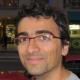
\includegraphics[width=0.6\columnwidth]{photo.jpg}\\[\baselineskip] % Your photo
\small % Smaller font size
Álvaro González \\ % Your name
\url{alvaroga@gmail.com} \\ % Your email address
+41 762 937 824 \\ % Your phone number
\Sep % Some whitespace
\textbf{Address} \\
Avenue D'Aïre 93F \\ % Address 1
Geneve, 1203 \\ % Address 2
\textbf{Nationality} \\
	Spanish 
\includegraphics{spain.png}\\ % Nationality
\vfill % Whitespace under this block to push it up under the photo
\end{flushright}
}

%----------------------------------------------------------------------------------------

\begin{document}

\userinformation % Print your information in the left column

\framebreak % End of the first column

%----------------------------------------------------------------------------------------
%	HEADING
%----------------------------------------------------------------------------------------

\cvheading{Álvaro González Álvarez} % Large heading - your name

\cvsubheading{Service Manager} % Subheading - your occupation/specialization

%----------------------------------------------------------------------------------------
%	ABOUT ME
%----------------------------------------------------------------------------------------

\aboutme{About Me}{I have worked at CERN in a DevOps position for the last 10 years. I have designed, implemented, integrated, maintained, and managed Linux based services.
I have worked with puppet based VMs, and now Kubernetes containers. I give technical support to teams and individuals. Provided version control, CI, and project management tools to a wide scientific community.
I have worked with people from more than 10 European countries, from Spain to Finland, from England to Greece.}
%----------------------------------------------------------------------------------------
%	COMPETENCES
%----------------------------------------------------------------------------------------

\CVSection{Competences} % From the competency model

{\begin{tabular}{p{0.23\textwidth} p{0.23\textwidth} p{0.23\textwidth}}
\bluebullet Managing self & \bluebullet Achieving results & \bluebullet Learning and Sharing Knowledge\\
\bluebullet Solution architecture & \bluebullet Application support & \bluebullet Problem management
\end{tabular}}

\CVSection{Experience}

%------------------------------------------------

\CVItem{October 2008 - November 2019, \textit{DevOps Engineer}, CERN}

\:
\:

\begin{itemize}
    \item Part of the developer services team. Using Linux for all the infrastructure. We have provided along the years services based in different technologies. Our version control offer was first CVS, then Subversion, and finally Git. In addition several JIRA instances were provided, a general purpose one, and some others for specific teams. For continuous integration and continuous delivery Jenkins, and GitLab CI are offered. Both deployed in an Openshift cluster that later was opened to the whole community.
\end{itemize}

\CVItem{November 2007 - September 2008, \textit{Procurement, Research, and Development IT Engineer}, Herca}{
\begin{itemize}
	\item Herca was a small startup company decided to build and operate a smart hotel. As the only IT in the company, I was in charge of the procurement of the IT material, install and configure it, develop the website, etc 
\end{itemize}
}

%------------------------------------------------

\Sep % Extra white space after the end of a major section

\CVSection{Technologies}

\begin{itemize}
\item Python Django Bash Java Perl
\item Quattor Puppet Ansible Kubernetes Openshift
\item Jira Bamboo Gitlab Subversion CVS Flexnet Jenkins WebSVN Trac
\item Nginx Apache Docker SAML OAuth PostgreSQL SQLite Oracle curl openssl Bootstrap PaaS
\item  Centos Red Hat Enterprise Linux Scientific Linux Fedora Atomic Debian Ubuntu
\end{itemize}

\clearpage % Start a new page
\userinformation % Print your information in the left column
\framebreak % End of the first columN

%----------------------------------------------------------------------------------------
%	Education
%----------------------------------------------------------------------------------------

\CVSection{Education}

\CVItem{University}{
\begin{itemize}
	\item October 2000 - September 2004, \textit{Universidad de Oviedo, Spain}. Bachelor.
	\item August 2005 - December 2005, \textit{University of North Carolina, USA} Exchange studinet.
	\item October 2004 - September 2007, \textit{Universidad de Oviedo, Spain}. Master.
\end{itemize}
}

\CVItem{Languages}

{\begin{tabular}{p{0.3\textwidth} p{0.4\textwidth}}
	\bluebullet Spanish, Native &  \bluebullet English, Fluent (C1) \\
	\bluebullet French, Intermediate (B1) \\
\end{tabular}}

\CVItem{Trainings}{
\begin{itemize}
        \item 2009-2010, General and Professional French courses
	\item 2009, Developing secure software
	\item 2009, Secure coding for Perl
	\item 2011, Communicating to Convince
	\item 2014, Making presentations
	\item 2015, Object-oriented Design Patterns
        \item 2015, Personal Awareness \& Impact
        \item 2016, Balancing Performance and Pressure
\end{itemize}
}

\CVItem{Conferences}{
\begin{itemize}
    \item HEPIX 2011, Darmstadt, Germany.
    \item CHEP 2012, New York, USA.
    \item HEPIX 2013, Bologna, Italy.
    \item HEPIX 2014, Annecy, France.
\end{itemize}}
%------------------------------------------------

\Sep

\end{document}
